% mainfile: ../../../../master.tex
\subsection{AOSP}
\label{task:20231114_aosp}

\subsubsection*{Zygote}
{Zygote} initializes by pre-loading the entire Android framework. Unlike desktop Java, it does not load the libraries lazily; it loads all of them as part of system start up. After completely initializing, it enters a tight loop, waiting for connections to a socket. When the system needs to create a new application, it connects to the Zygote socket and sends a small packet describing the application to be started. Zygote clones itself, creating a new kernel-level process.

Memory is organized into uniformly sized \textbf{pages}. When the application refers to memory at a particular address, the device hardware reinterprets the address as an index into a \textbf{page table}. Newly cloned Zygote processes for newly started applications are simply clone of Zygote's page table, pointing to the exact same pages of physical memory. Only the pages the new application uses for its own purposes are not shared:

\begin{figure}[H]
    \centering
    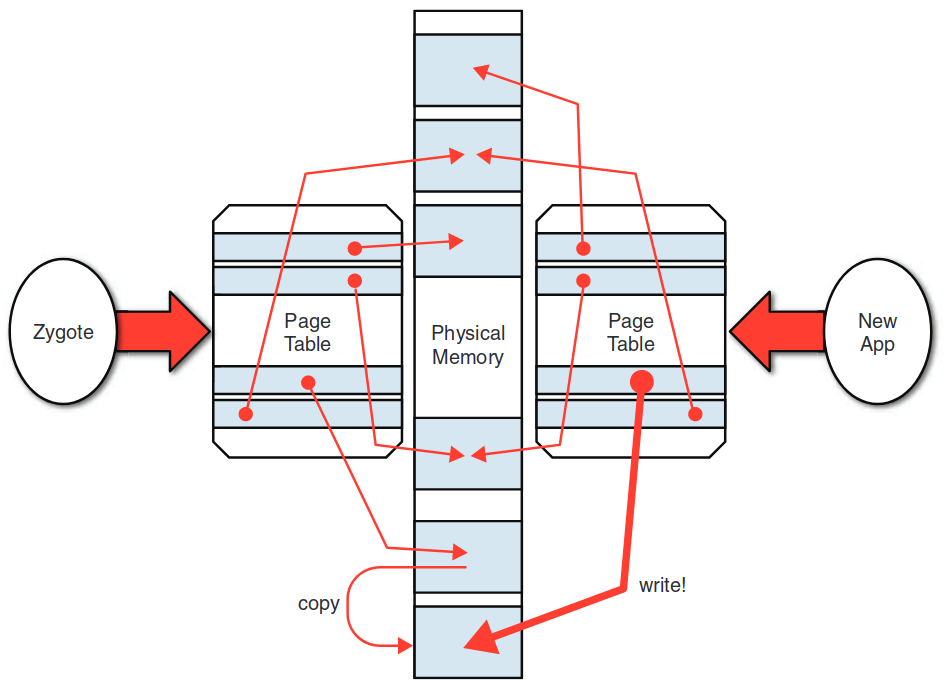
\includegraphics[width=.75\linewidth]{entries/2023/11/14/copyonwrite.png}
    \caption{Zygote Copy-on Write}
    \label{fig:copyonwrite}
\end{figure}

\subsubsection*{Zygote Initialization}

Zygote is started by \texttt{init}. \texttt{ro.zygote} system variable set at platform build time decides which of four types of Zygotes are started and which one is "primary". Both the \texttt{init} and Zygote scripts are stored inside \texttt{\$AOSP/system/core/rootdir}. In the following \texttt{init.zygote64\_32.rc}, 2 Zygote processes, primary and secondary, are started at 2 different sockets:

\begin{lstlisting}
service zygote /system/bin/app_process64 -Xzygote \
        /system/bin --zygote --start-system-server --socket-name=zygote
    class main
    priority -20
    user root
    group root readproc reserved_disk
    socket zygote stream 660 root system
    socket usap_pool_primary stream 660 root system
    onrestart exec_background - system system -- /system/bin/vdc volume abort_fuse
    onrestart write /sys/power/state on
    onrestart restart audioserver
    onrestart restart cameraserver
    onrestart restart media
    onrestart restart media.tuner
    onrestart restart netd
    onrestart restart wificond
    task_profiles ProcessCapacityHigh MaxPerformance
    critical window=${zygote.critical_window.minute:-off} target=zygote-fatal

service zygote_secondary /system/bin/app_process32 -Xzygote \
        /system/bin --zygote --socket-name=zygote_secondary --enable-lazy-preload
    class main
    priority -20
    user root
    group root readproc reserved_disk
    socket zygote_secondary stream 660 root system
    socket usap_pool_secondary stream 660 root system
    onrestart restart zygote
    task_profiles ProcessCapacityHigh MaxPerformance
    disabled
\end{lstlisting}

The actual application that is started as user root at the very highest priority by \texttt{init} is \texttt{/system/bin/app\_process64}. The script requests that \texttt{init} create a stream socket for the process and catalog it as \texttt{/dev/socket/zygote\_secondary} which will be used by the system to start new Android applications.

Zygote is only started once during the system startup, by \texttt{app\_process64} and \texttt{app\_process32}, and is simply cloned to start subsequent applications. Zygote initialization sequence is described below:
\begin{longtable}{p{.25\linewidth}  p{.50\linewidth} p{.25\linewidth}} 
\toprule
Method 	& Description & Source\\
\midrule

\texttt{\textbf{init.rc}} 
&Imports the \texttt{init.zygote64\_32.rc} that contains the script that starts Zygote service.
&\texttt{\$AOSP/system/core/rootdir}\\

\texttt{\textbf{init.zygote64\_32.rc}} 
&Runs \texttt{app\_process64} and \texttt{app\_process32} which will initialize the starting of Zygote service.
&\texttt{\$AOSP/system/core/rootdir}\\

\texttt{\textbf{app\_process}} 
&Creates \texttt{AppRuntime}, a subclass of \texttt{AndroidRuntime}, that does bookkeeping, naming the process, setting up parameter, and the name of the class to run when not running Zygote, and then calls \texttt{AndroidRuntime.start()} to invoke the runtime.
&\texttt{\$AOSP/frameworks/base/cmds/app\_process}\\

\texttt{\textbf{AppRuntime::start}} 
&Invokes \texttt{startVM} which invokes \texttt{JNI\_CreateJavaVM}.
&\url{AOSP/frameworks/base/core/jni/AndroidRuntime.cpp}\\

\texttt{\textbf{JNI\_CreateJavaVM}} 
&Calls \texttt{Runtime::Create}.
&\texttt{\$AOSP/art/runtime/jni/java\_vm\_ext.cc}\\

\texttt{\textbf{Runtime::Create}} 
&Initializes the ART runtime, loading the system OAT files and the libraries they contain.
&\texttt{\$AOSP/art/runtime/runtime.cc}\\

\midrule
\caption{Zygote Initialization Sequence} 
\label{tab:zygoteinitializationsequence}
\end{longtable}

The argument that \texttt{app\_process} passed to \texttt{start} is \texttt{com.android.internal.os.Zygote.Init}, the source for which is in \texttt{\$AOSP/frameworks/base/core/java/com/android/internal/os/ZygoteInit.java}. \texttt{app\_process} is the launcher for all Java programs (not apps!) in the Android system, and Zygote is one example of the programs (system service) to be launched.

\subsubsection*{Zygote System Service}

Zygote has 3 major tasks, on startup:
\begin{enumerate}
    \item Register the socket to which the system will connect to start new application. Handled by \texttt{registerServerSocket} method which creates socket using the named passed as parameter for \texttt{init} script.
    \item Preload Android resources (classes, libraries, resources and even WebViews) with a call to \texttt{preload} method. After \texttt{preload} is finished, Zygote is fully initialized and ready to clone to new applications very quickly.
    \item Start Android System Server. Thus, \texttt{SystemServer} is the first application to be cloned by Zygote.
\end{enumerate}
After it has completed these three tasks, it enters a loop, waiting for connections to the socket.
